\section{Derivatives}

In addition to tasks that require an accurate function in the RMSE sense, tasks that concern with
the computation of derivative quantities such as gradient and Laplacian are of fundamental
importance in data analysis. As such, in this section we study streams that minimize gradient and
Laplacian errors. For the experiments in this section, we use the 4-4 B-spline wavelet [CITE] that
has four vanishing moments on each of the analysis and synthesis sides, to ensure that the
reconstructed function is smooth enough for the purpose of taking derivatives.

\subsection{Gradient}

We use the three-point central difference formula for computing partial derivatives in each
direction: $\frac{\partial f}{\partial x}\approx \frac{f(x+1)-f(x-1)}{2}$, and the same for $y$. The
gradient at each point ($\nabla f(x,y)$) is the vector $(\frac{\partial f}{\partial
x},\frac{\partial f}{\partial y})$. The difference between the gradient of a reconstructed function
using $b$ bits per sample $f_b$ and the original function $f$ is defined as $\norm{\nabla f_b-\nabla
f}_2$. For each data set, we use algorithm [CITE] to compute a stream that minimizes this difference
at any $b$, and call it the \emph{gradient-optimized} stream. Figure
\ref{fig:gradient-error-comparison} compares the \emph{gradient-optimized} with the
\emph{rmse-optimized} streams for four data sets.

\begin{figure}
	\centering
	\subcaptionbox{euler}
	{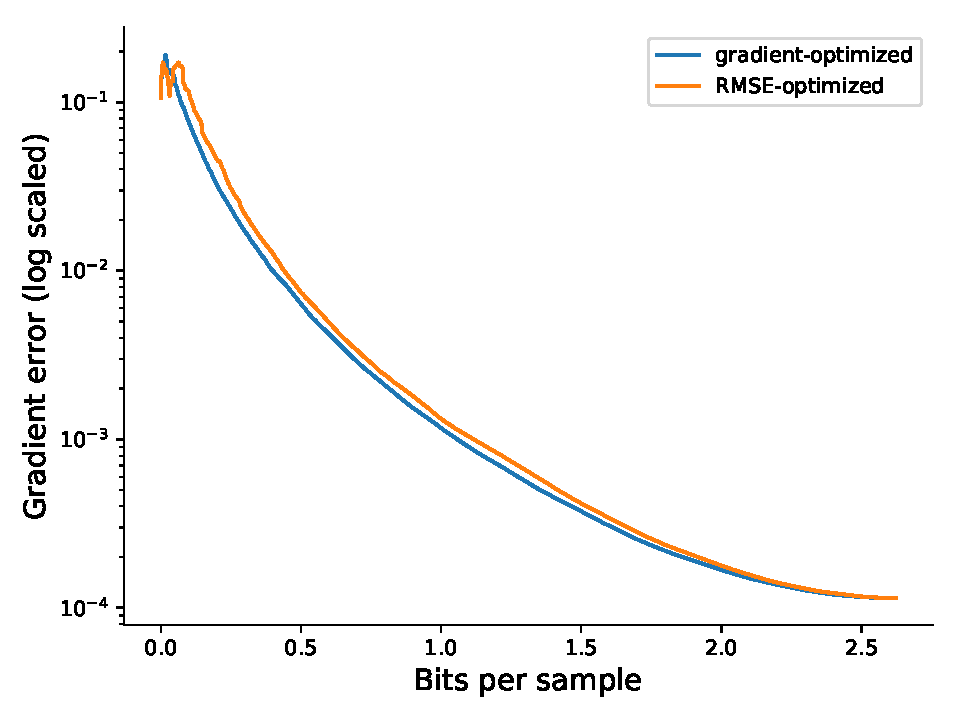
\includegraphics[width=0.48\linewidth]{img/gradient-laplacian/euler-gradient.pdf}}
	\subcaptionbox{magnetic}
	{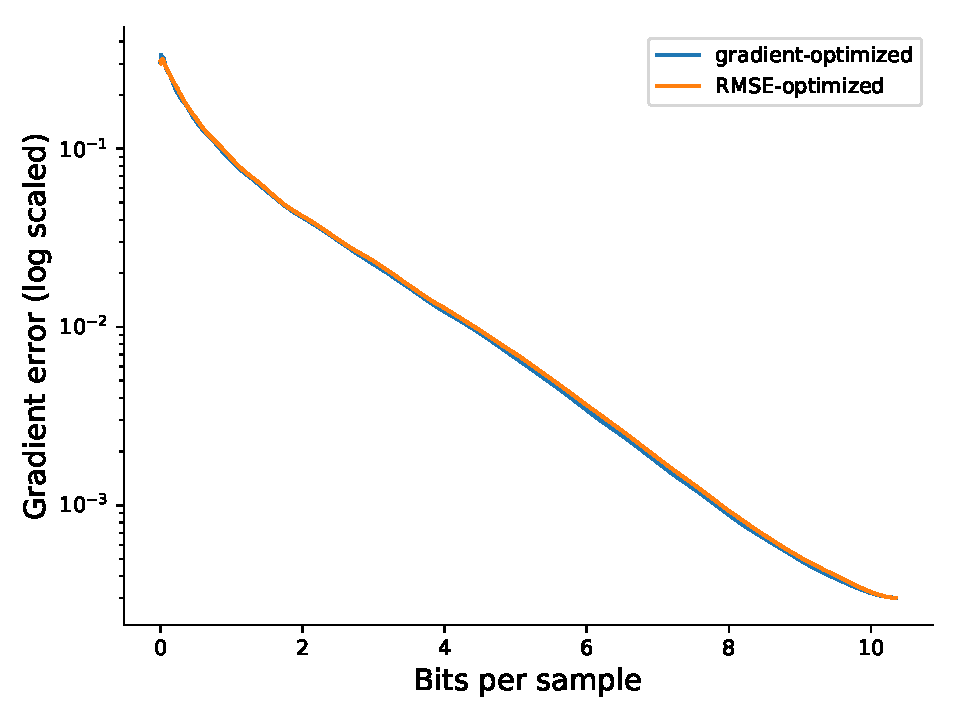
\includegraphics[width=0.48\linewidth]{img/gradient-laplacian/magnetic-gradient.pdf}}
	\subcaptionbox{diffusivity}
	{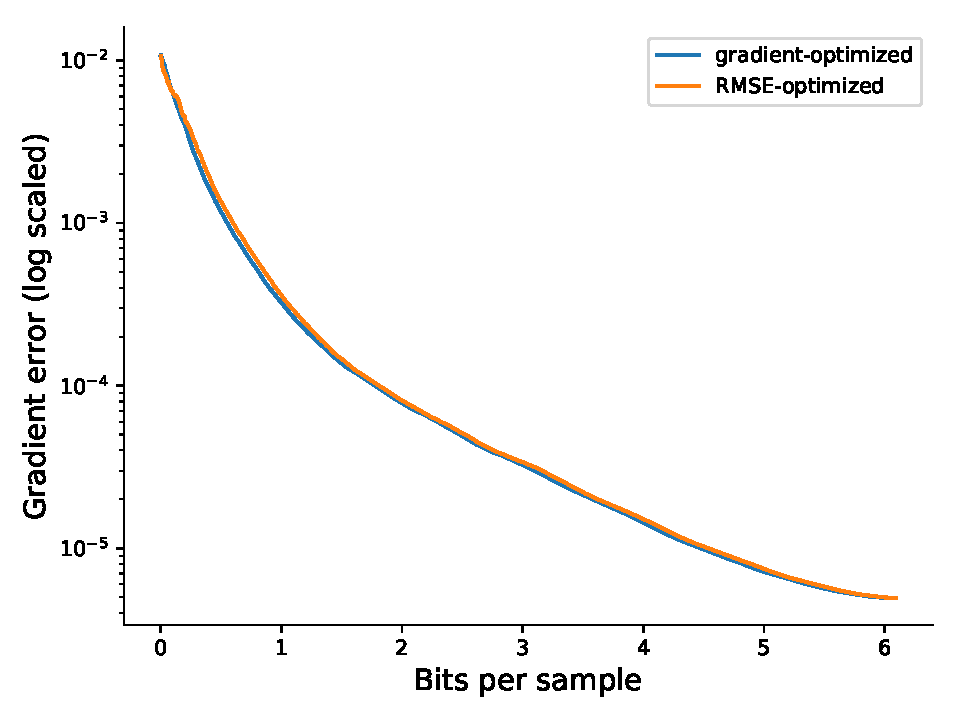
\includegraphics[width=0.48\linewidth]{img/gradient-laplacian/miranda-diffusivity-gradient.pdf}}
	\subcaptionbox{velocityx}
	{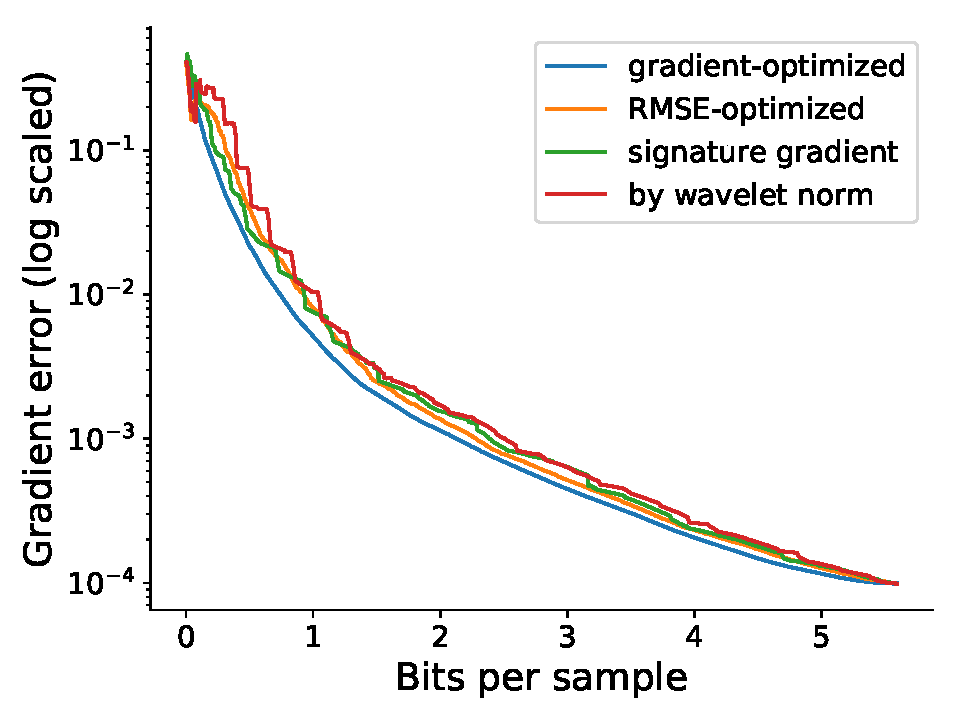
\includegraphics[width=0.48\linewidth]{img/gradient-laplacian/miranda-velocityz-gradient.pdf}}
	\caption{Gradient error comparison between \emph{gradient-optimized} and \emph{rmse-optimized}
	streams for four data sets. Note that the leading zero chunks are still skipped.}
	\label{fig:gradient-error-comparison}
\end{figure}

Figure \ref{fig:gradient-error-comparison} suggests that the \emph{rmse-optimized} streams are also
nearly optimal for gradient computation. The linear gradient operator resulting from the three-point
finite difference formula is not invertible, that is, there are infinitely many functions that
result in the same gradient field. So it is not surprising that the two streams both produce the
best possible gradient progression, but it is worth noting that only the \emph{rmse-optimized}
stream produces an accurate function as well. We give evidence to this claim is in Figure
\ref{fig:gradient-comparison}, in which we reconstruct the euler data at 0.25 bits per sample using
both streams, and show the difference in gradient between the two. The two gradient fields differ
the most along very sharp edges, but are in general in congruent (a), while the
\emph{rmse-optimized} stream produces significantly more accurate reconstruction of the function
itself (b, c, and d).

\begin{figure}
	\centering
	\subcaptionbox{gradient difference}
	{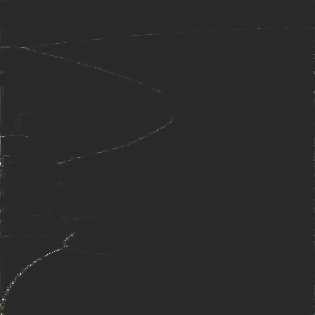
\includegraphics[width=0.24\linewidth]{img/gradient-laplacian/grad-diff.png}}
	\subcaptionbox{original data}
	{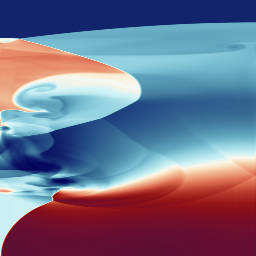
\includegraphics[width=0.24\linewidth]{img/gradient-laplacian/euler-original.png}}
	\subcaptionbox{\emph{rmse-optimized}}
	{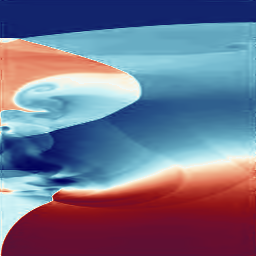
\includegraphics[width=0.24\linewidth]{img/gradient-laplacian/euler-rmse.png}}
	\subcaptionbox{\emph{gradient-optimized}}
	{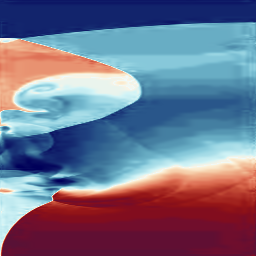
\includegraphics[width=0.24\linewidth]{img/gradient-laplacian/euler-gradient.png}}
	\caption{Comparing \emph{rmse-optimized} and \emph{gradient-optimized} at 0.25 bits per sample. }
	\label{fig:gradient-comparison}
\end{figure}

It is therefore reasonable in practice to simply use heuristics that are optimized for RMSE when the
analysis relies on an accurate gradient field. One such heuristic is the one used by the \emph{by
wavelet norm} stream (when coupled with a typical entropy compression that avoids most of the
leading zero bits).

\subsection{Laplacian}

Figure 2: Laplacian difference between Laplacian and rmse

Figure 3: PSNR plot for gradient, laplacian and rmse streams

We conclude that the rmse strea subsumes gradient and laplacian
